
\documentclass{article}
\usepackage[a2paper, margin=1cm]{geometry}
\usepackage{tikz}
\begin{document}
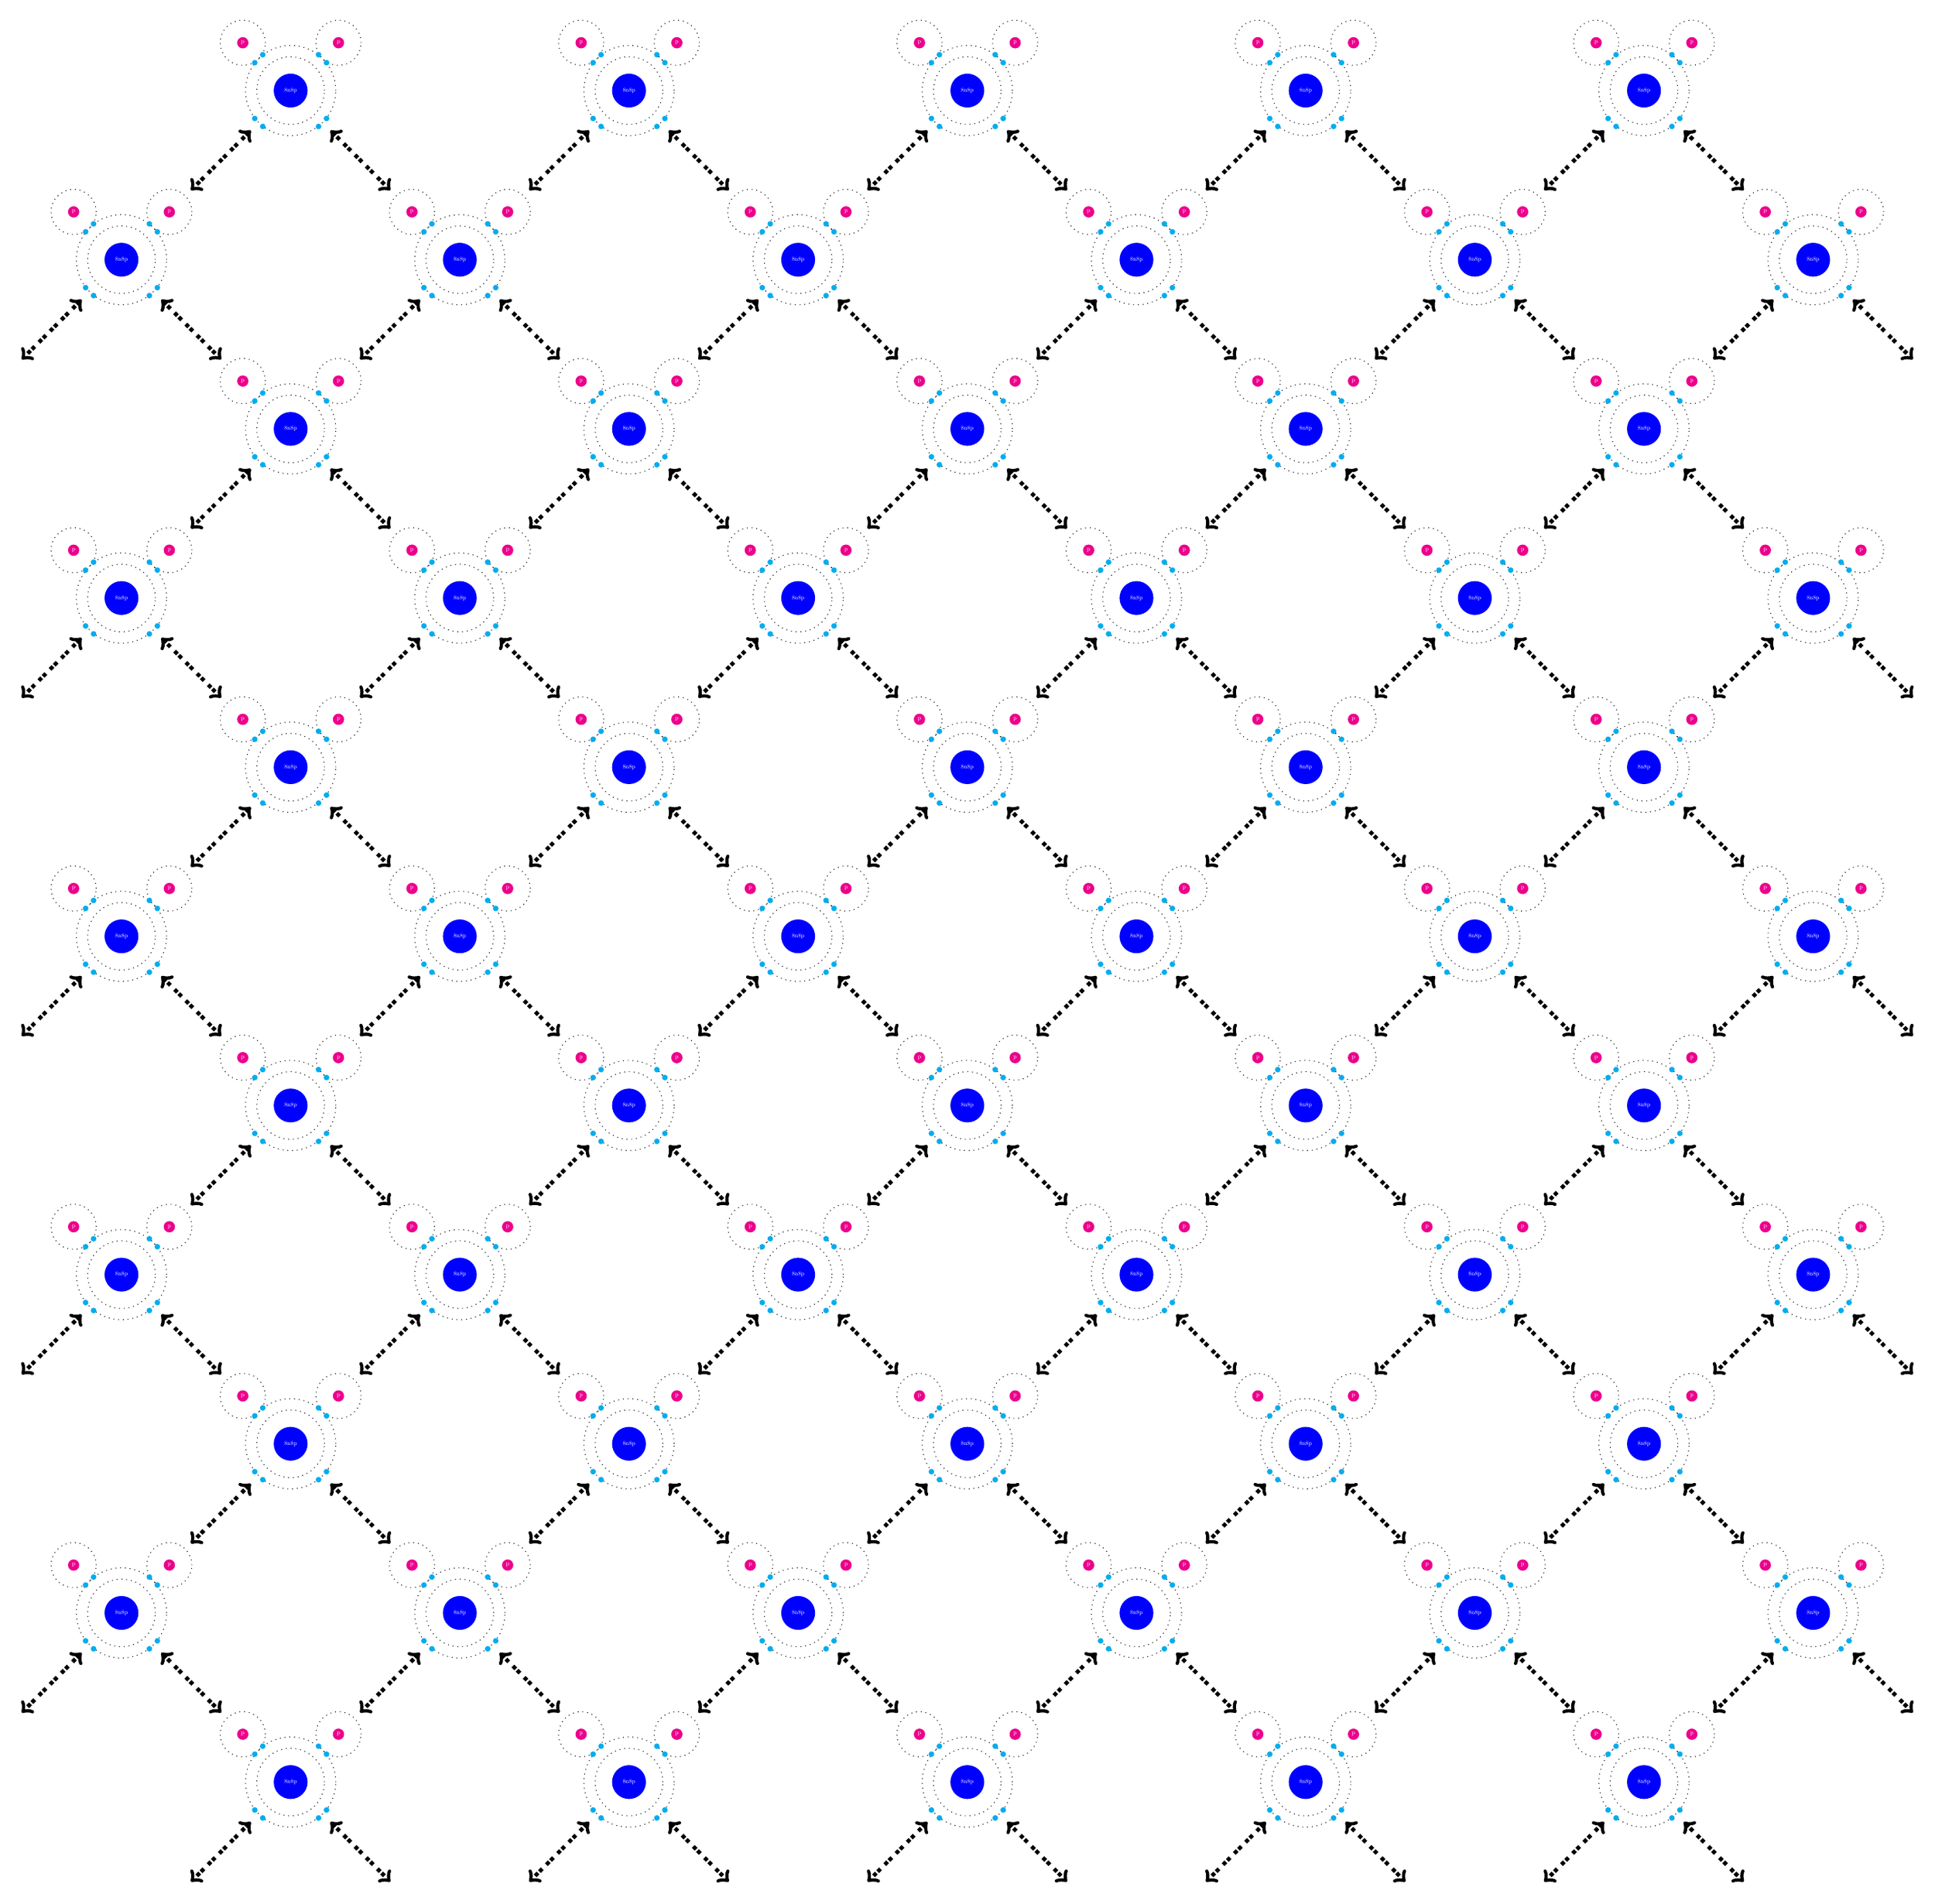
\begin{tikzpicture}
    \foreach \x in {0, ..., 10} {
        \foreach \y in {0, ..., 10} {
            \ifodd\numexpr\x+\y\relax
            \tikzset{shift={(\x*3, \y*3)}}
            \fill [blue] (0, 0) circle (0.3) node [white, scale=0.3] {8n8p};
            \fill [magenta]
                (45:1.2) circle (0.1) node [white, scale=0.3] {p}
                [magenta] (135:1.2) circle (0.1) node [white, scale=0.3] {p}
            ;
            \draw [dotted] (0, 0) circle (0.6) circle (0.8);
            \draw [dotted] (45:1.2) circle (0.4) (135:1.2) circle (0.4);
            \fill [cyan]
                (45:0.8) +(-45:0.1) circle (0.05) +(135:0.1) circle (0.05)
                (135:0.8) +(45:0.1) circle (0.05) +(-135:0.1) circle (0.05)
                (-135:0.8) +(-45:0.1) circle (0.05) +(135:0.1) circle (0.05)
                (-45:0.8) +(45:0.1) circle (0.05) +(-135:0.1) circle (0.05)
            ;
            \draw [dash pattern=on2pt off1pt on2pt off3pt, <->, line width=2pt]
                (-45:1) -- (-45:2.5);
            \draw [dash pattern=on2pt off1pt on2pt off3pt, <->, line width=2pt]
                (-135:1) -- (-135:2.5);
            \fi
        }
    }
\end{tikzpicture}
\end{document}

